\documentclass[12pt]{article}
\usepackage[utf8]{inputenc}
\usepackage{amsmath}
\usepackage{graphicx}
\usepackage{geometry}
\geometry{a4paper, margin=1in}
\usepackage{xcolor}
\usepackage{listings}
\usepackage{hyperref}

% Define style for code listings
\definecolor{codegray}{rgb}{0.5,0.5,0.5}
\definecolor{backcolour}{rgb}{0.95,0.95,0.92}
\lstdefinestyle{mystyle}{
    backgroundcolor=\color{backcolour},   
    commentstyle=\color{codegray},
    keywordstyle=\color{blue},
    numberstyle=\tiny\color{codegray},
    stringstyle=\color{magenta},
    basicstyle=\ttfamily\footnotesize,
    breaklines=true,                 
    breakatwhitespace=false,         
    captionpos=b,
    keepspaces=true,
    numbers=left,                    
    numbersep=5pt,
    showspaces=false,
    showstringspaces=false,
    showtabs=false,
    tabsize=2
}
\lstset{style=mystyle}

\title{\textbf{ME302: 2024-25 - II} \\ \textbf{COURSE PROJECT REPORT}}
\author{%
    Navnit Patel (220701),
    Devraj Mathur (220349),
    Himanshu Singh (220455)}
\date{}

\begin{document}

\maketitle

\section*{\large{1. PROBLEM DESCRIPTION}}
This project aims to determine the optimum model scaling factor to test a turbomachine component in a closed-loop high-pressure flow facility. In order to accurately simulate the full-scale prototype, the scaled model must match both the Mach and Reynolds numbers of the target engine conditions. The model scale is defined as
\[
\text{scale} = \frac{l_{\text{model}}}{l_{\text{prototype}}},
\]
with \(l_{\text{prototype}} = 0.2\,\text{m}\). The compressor inlet conditions are specified as \(T_{01}=293\,\text{K}\), while the inlet pressure \(p_{01}\) is initially unknown and is determined through the analysis. Moreover, the test must meet the facility constraint that no pressure anywhere exceeds 250 kPa and satisfy the closed-loop condition \(p_{05} \ge p_{01}\) (with \(p_{05}=0.95\,p_{04}\) and \(p_{04}=0.985\,p_{02}\)). The compressor performance is characterized by its reference mass flow rate, the temperature ratio \(T_{02}/T_{01}\), and the pressure ratio \(p_{02}/p_{01}\). The test section inlet diameter is assumed to be \(D_4 = 2\,l_{\text{model}}\) to provide sufficient space for instrumentation.

\section*{\large{2. METHODOLOGY}}
The analysis is performed by computing key parameters at the test section (station 4) using the following steps:

\begin{enumerate}
    \item \textbf{ Compressor Inlet Conditions:} \\
    The compressor inlet total temperature \(T_{01}\) is fixed at 293 K. However, the inlet pressure \(p_{01}\) is not known a priori and is determined via:
    \[
    p_{01} = \frac{p_{02}}{p0\_ratio}.
    \]

    \item \textbf{Compressor Exit Conditions:} \\
    The stagnation conditions after the compressor are:
    \[
    T_{02} = \texttt{T0\_ratio} \times T_{01}, \quad p_{02} = \texttt{p0\_ratio} \times p_{01}.
    \]

    \item \textbf{Diffuser Inlet and Exit Conditions:} \\
    Flow from the compressor enters the diffuser at station 3 and exits at station 4 (test section). Under the conditions:
    \begin{itemize}
        \item At the diffuser inlet (station 3):
        \[
        T_{03} = T_{02}, \quad p_{03} = 0.985\,p_{02}.
        \]
        \item Assuming negligible viscous losses, the diffuser exit (station 4) conditions are:
        \[
        T_{04} = T_{03}, \quad p_{04} = p_{03}.
        \]
        These values serve as input to the isentropic relations used to determine static conditions at station 4.
    \end{itemize}
 
    \item \textbf{Static Flow Conditions:} \\
    The static temperature at station 4 is:
    \[
    T_{4} = \frac{T_{04}}{1+\frac{\gamma-1}{2}M_{\text{target}}^2},
    \]
    and the local speed of sound and flow velocity are:
    \[
    a_{4} = \sqrt{\gamma R T_{4}}, \quad V_{4} = M_{\text{target}}\,a_{4},
    \]
    where \(M_{\text{target}}=0.55\), \(\gamma = 1.4\), and \(R = 287\,\text{J/(kg\,K)}\).
        % \item \textbf{Stagnation and Compressor Pressures:} \\
    The stagnation pressure at station 4 is recovered via:
    \[
    p_{04} = p_{4}\left(1+\frac{\gamma-1}{2}M_{\text{target}}^2\right)^{\frac{\gamma}{\gamma-1}},
    \]
    and the compressor exit pressure is:
    \[
    p_{02} = \frac{p_{04}}{0.985},
    \]
    with the inlet stagnation pressure computed as:
    \[
    p_{01} = \frac{p_{02}}{p0\_ratio}.
    \]
    \item \textbf{Reynolds Number and Density Calculation:} \\
    To ensure dynamic similarity, the local density is computed from the Reynolds number relation:
    \[
    \rho_{4} = \frac{Re\,\mu}{V_{4}\,l_{\text{model}}},
    \]
    which is then used in the ideal gas law to calculate the static pressure at station 4:
    \[
    p_{4} = \frac{\rho_{4}\,R\,T_{4}}{1000}\quad\text{(in kPa)}.
    \]
    where \(Re = 3\times10^6\) and \(\mu = 1.83\times10^{-5}\).
    \item \textbf{Maximum Scale Calculation:} \\
    Based on mass flow and geometry, the mass flow in the test section is expressed as:
   \[
\dot{m} = \rho_{4} V_{4} A_{4} = \rho_{4} V_{4} \pi\, l_{\text{model}}^{2}
\]
\[
\dot{m} = \dot{m}_{\text{ref}} \cdot \frac{p_{01}}{101325} \cdot \sqrt{\frac{T_{01}}{293}}
\]
where \( T_{01} = 293\,\text{K} \) and \( p_{01} \) is in Pascals.

Equating the supplied mass flow (from the compressor, adjusted to reference conditions) to the test section mass flow and solving for the scale yields:

    \[
    \text{scale}_{\text{max}} = \sqrt{\frac{\dot{m}}{\rho_{4}V_{4}\pi\,l_{\text{prototype}}^{2}},
    }
    \]
    which, after simplification and incorporating the reference pressure, is given by:
\[
\text{scale}_{\text{max}} = \sqrt{ \frac{ \dot{m}_{\text{ref}} \, R \, T_{4} }{ 0.985 \, p0\_ratio \, V_{4} \, \pi \, \left(1 + \frac{\gamma - 1}{2} M_{\text{target}}^2\right)^{\frac{\gamma}{\gamma - 1}} \, l_{\text{prototype}}^{2} \cdot 101325 } }
\]

    and the corresponding model length is:
    \[
    l_{\text{model}} = \text{scale}_{\text{max}}\,l_{\text{prototype}}.
    \]


    


    \item \textbf{Closed-Loop Operation:} \\
For the facility to operate in a closed loop, the final pressure \( p_{05} \) must not fall below the inlet pressure:
\[
p_{05} \ge p_{01}.
\]
Substituting the expressions, we have:
\[
p_{05} = 0.95 \, p_{04} = 0.95 \times 0.985 \, p0\_ratio \, p_{01} = 0.93575 \, p0\_ratio \, p_{01}.
\]
Thus, the closed-loop condition requires:
\[
0.93575 \, p0\_ratio \, p_{01} \ge p_{01} \quad \Rightarrow \quad p0\_ratio \ge 1.068.
\]
The compressor data confirms that this condition is satisfied.

    \item \textbf{Feasibility Criteria:} \\
    The operating point is deemed acceptable if:
    \[
    \text{scale}_{\text{max}} \le 1 \quad \text{and} \quad p_{02} \le 250\,\text{kPa}.
    \]
    since station 2 is subjected to the maximum pressure constraint.
\end{enumerate}

\section*{\large{3. RESULTS AND DISCUSSION}}

\subsection*{Results}
The analysis yields the following optimal operating point:
\begin{itemize}
    \item \textbf{Maximum Scale:} 0.6179
    \item \textbf{Inlet Stagnation Pressure, \(p_{01}\):} 204.70 kPa
    \item \textbf{Compressor Map Pressure Ratio, \(p0\_ratio\):} 1.2105
    \item \textbf{Compressor Exit Stagnation Pressure, \(p_{02}\):} 247.78 kPa
    \item \textbf{Reference Mass Flow, \(\dot{m}_{\text{ref}}\):} 10.5503 kg/s
    \item \(\theta = \arctan\left(\frac{(D_4-D_3)}{2L}\right) = -6.7080^\circ\)
\end{itemize}

Here, the inlet diameter of the test section is calculated as \(D_4 = 2\,l_{\text{model}}\), while the diffuser inlet diameter \(D_3\) is known. The computed values satisfy the closed-loop requirement \(p_{05} \ge p_{01}\). Additionally, since the diffuser angle \(\theta\) is negative, the assumption of negligible losses is justified.

\subsection*{Discussion}
By enforcing both mass flow rate and Reynolds number constraints, the analysis successfully identifies a unique operating point that achieves the maximum permissible model scale while maintaining dynamic similarity with the prototype. The determined scale of approximately 0.6179 indicates that the model length (\(l_{\text{model}}\)) is nearly 61.79\% of the original prototype length. The corresponding inlet stagnation pressure of around 205 kPa ensures that the resulting compressor exit pressure remains within the facility’s upper limit of 250 kPa.

\begin{figure}[h]
    \centering
    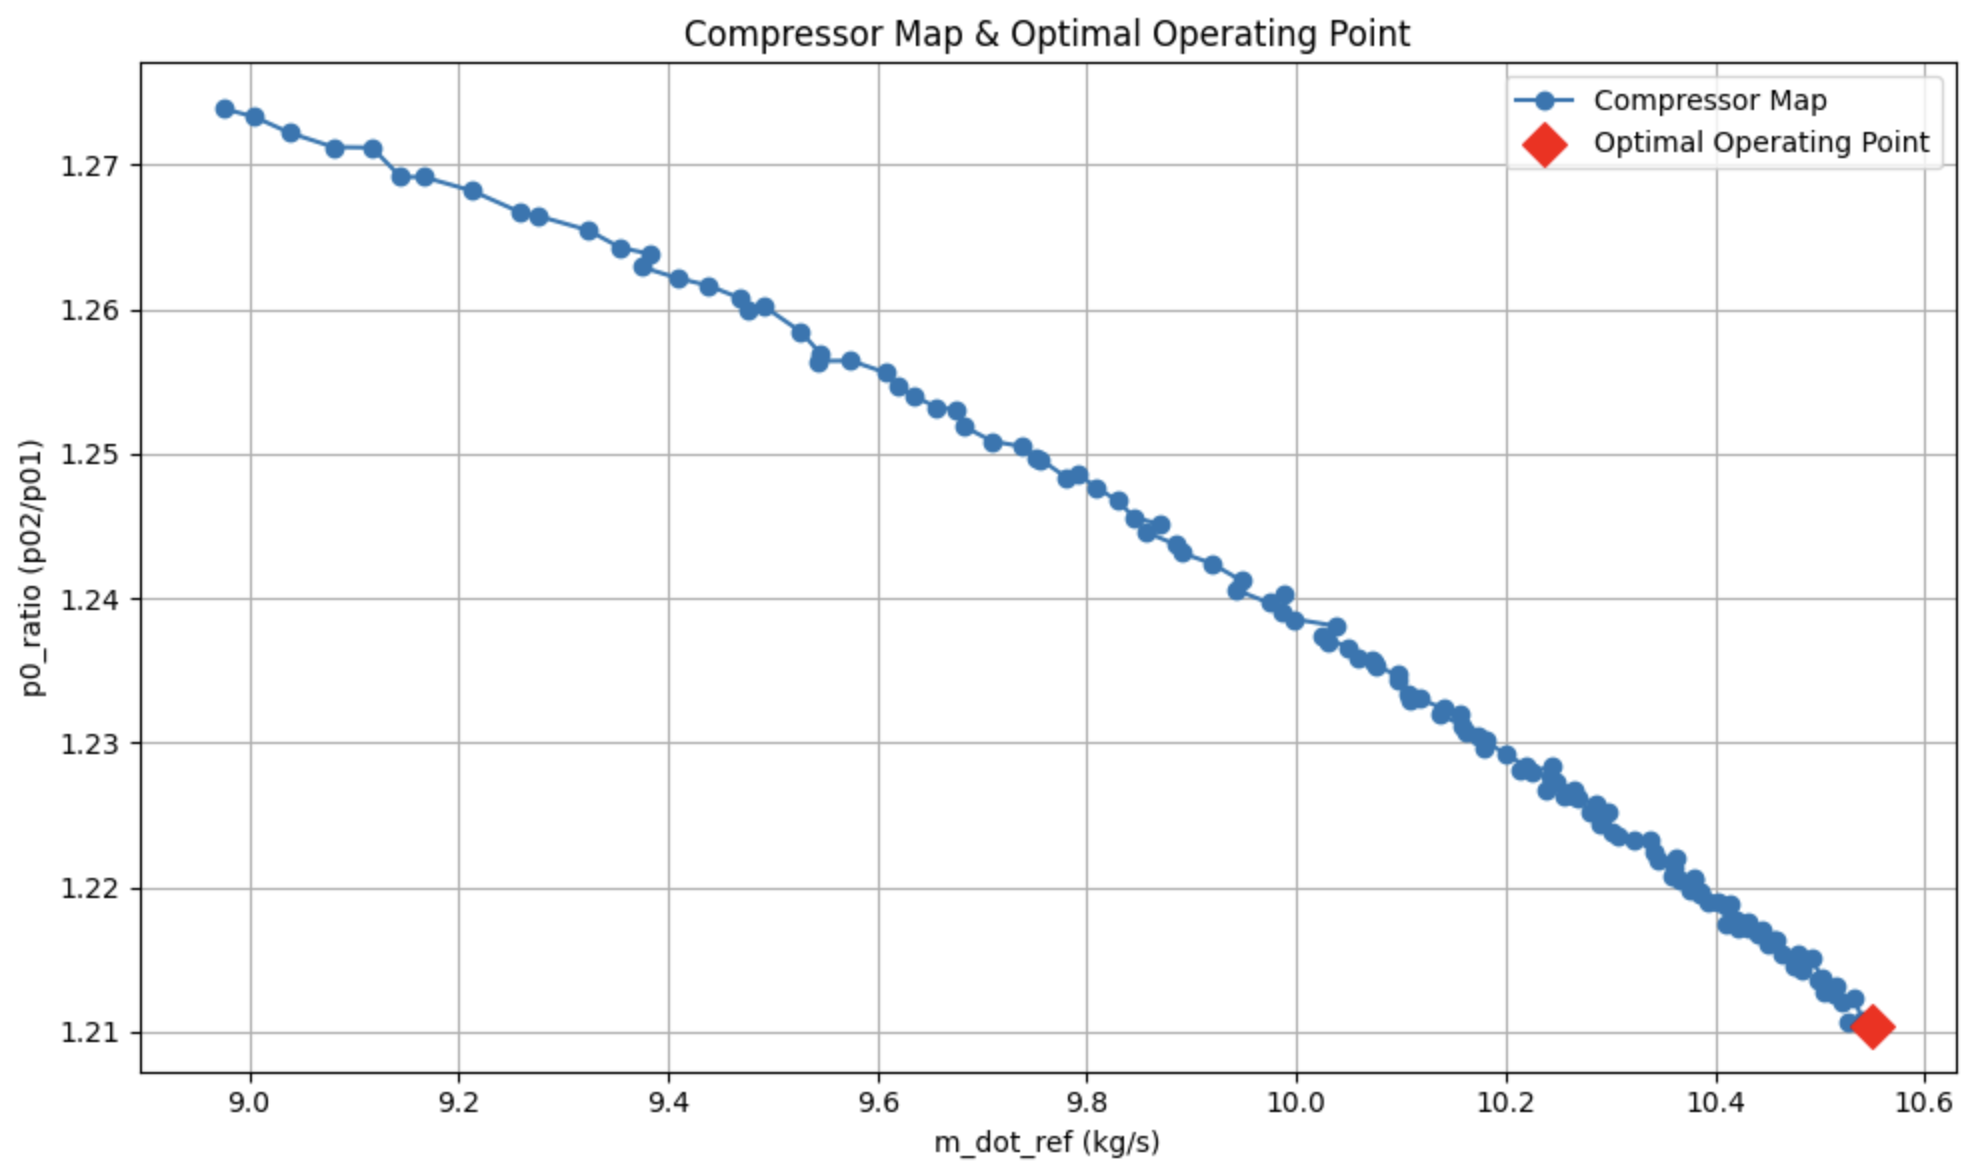
\includegraphics[width=1.0\textwidth]{compressor_map.png} % Increased the width from 0.8 to 1.0
    \caption{Compressor operation map (\(p_0\) ratio vs. \(\dot{m}_{\text{ref}}\)) showing the selected optimal operating point in red.}
    \label{fig:compressor-map}
\end{figure}

As shown in Figure~\ref{fig:compressor-map}, the compressor map highlights the chosen optimal operating point. These results confirm that the adopted approach effectively determines a model configuration that replicates the flow physics of the full-scale prototype while complying with the operational limits of the test facility.
\section*{\large{5. FUTURE WORK}}
Based on the proven testing methodology, future investigations can be carried out by solely modifying the test section and the upstream diffuser. The following three potential experimental research studies are proposed:
\subsection*{5.1 Flow Separation Control in Diffusers}
This research will explore both active and passive flow control strategies to reduce flow separation in the diffuser section. By utilizing the adjustable diffuser geometry available in the facility, various techniques—including vortex generators, plasma actuators, and synthetic jets—will be experimentally tested to enhance pressure recovery and improve flow uniformity over a range of divergence angles. The aim is to optimize diffuser performance and reduce aerodynamic losses, thereby increasing turbine efficiency and operational stability.  
\\\textbf{Potential Beneficiaries:} GE Vernova, Siemens Energy, Mitsubishi Power

\subsection*{5.2 Hydrogen Flow Behavior in Turbomachinery}
This study will modify the test section to enable safe and controlled experiments with hydrogen-rich flows. The objective is to investigate how increasing hydrogen content in the fuel mix affects flow characteristics, heat transfer, and material compatibility. By maintaining prototype-level Mach and Reynolds numbers in a closed-loop configuration, this research will provide critical data on the aerothermal behavior of hydrogen-fueled turbomachinery. The findings will be instrumental in developing turbines that can efficiently operate with high-hydrogen fuels.
\\\textbf{Potential Beneficiaries:} Siemens Energy, MAN Energy Solutions, Mitsubishi Power

\subsection*{5.3 Advanced Cooling Designs for High-Temperature Components}
This experiment will assess innovative cooling configurations for turbine components operating under high-temperature conditions. Scaled models of turbine blades featuring internal cooling passages and external film cooling schemes will be tested to measure surface temperature distributions and evaluate cooling effectiveness. The goal is to refine cooling strategies that maintain component integrity and enhance engine efficiency, addressing critical challenges related to high thermal loads.
\\\textbf{Potential Beneficiaries:} Aerospace firms and material science companies partnering with GTRE and global OEMs

\subsection*{Conclusion}
The proposed research directions take full advantage of the unique capabilities of the test facility while targeting key challenges in modern gas turbine technology. The studies on flow separation control, hydrogen flow behavior, and advanced cooling designs are each designed to yield actionable insights that can improve component performance and operational reliability. Collectively, these experiments could attract industrial partnerships and funding, advancing the development of next-generation turbomachinery that meets stringent efficiency and environmental standards.

\section*{\large{6. REFERENCES}}
\begin{itemize}
\item \href{https://dl.icdst.org/pdfs/files3/78256836a74743b12293cba5e27e4dc3.pdf}{\textit{Fluid Mechanics and Thermodynamics of Turbomachinery, 7th Edition by S. L. Dixon and C. A. Hall, Elsevier.}} 
\item \href{https://iopscience.iop.org/article/10.1088/1757-899X/1180/1/012041/pdf}{\textit{Development of accurate and widely applicable
compressor performance maps.}}
\item \href{https://www.sciencedirect.com/science/article/pii/S1270963823001347}{\textit{Flow separation control and performance evaluation of an asymmetric diffuser using vortex generators.}}
\item \href{https://asmedigitalcollection.asme.org/turbomachinery/article/147/7/071008/1208628/Targeting-Full-Hydrogen-Operation-on-Industrial}{\textit{Targeting Full-Hydrogen
Operation on Industrial-Scale Gas Turbines: Impact of Unconventional Fuels on
Turbine Module Performance and Aeromechanics.}}

\item \href{https://www.sciencedirect.com/science/article/pii/S2212540X2200044X}{\textit{ A review of cooling technologies for high temperature rotating components in gas turbine.}}

\end{itemize}

\section*{\large{7. SUPPLEMENT}}
The following files are attached with this report:
\begin{itemize}
    \item Python code: \href{https://github.com/Navnit1294/ME_302_Course_Project/edit/main/compressor_map.py#L23C0}{\texttt{compressor\_scale\_analysis.py}}
    \item LaTeX source file: \href{https://github.com/Navnit1294/ME_302_Course_Project/blob/main/ME_302_Course_Project.tex}{\texttt{project report.tex}}
    \item Compressor data (text format): \href{https://github.com/Navnit1294/ME_302_Course_Project/blob/main/Compressor_operation_map.txt}{\texttt{Compressor\_operation\_map.txt}}
    \item Compressor data (Excel format): \href{https://github.com/Navnit1294/ME_302_Course_Project/blob/main/Compressor_operation_map.xlsx}{\texttt{Compressor\_operation\_map.xlsx}}
\end{itemize}
\section*{\large{8. Python Instuction}}
Ensure that the data file Compressor\_operation\_map.txt is located in the same
directory as the Python script for proper execution.

\end{document}
